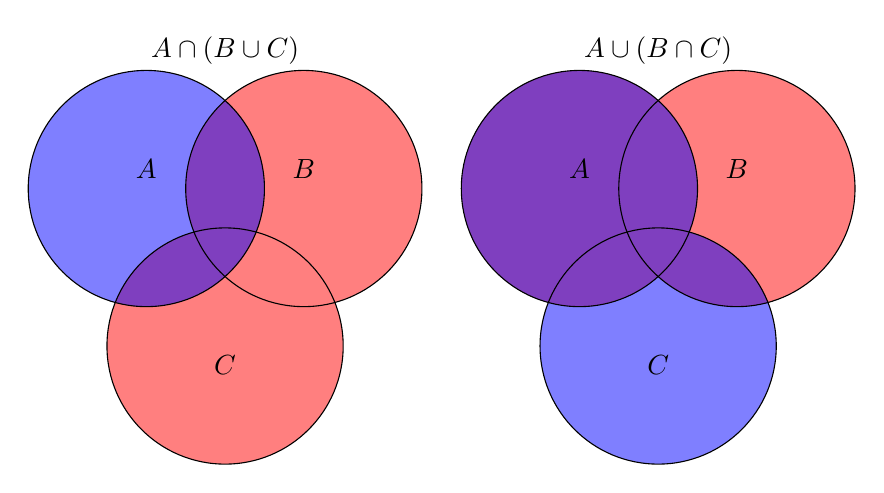
\begin{tikzpicture}[scale=0.5]
    \begin{scope}[xshift=5.5cm]
        \coordinate (A) at (-2,  2);
        \coordinate (B) at ( 2,  2);
        \coordinate (C) at ( 0, -2);

        \begin{scope}
            \clip (A) circle (3cm) (B) circle (3cm);
            \fill[red, opacity=0.5] (-5, -5) rectangle (5, 5);
        \end{scope}

        \begin{scope}
            \clip (A) circle (3cm) (C) circle (3cm);
            \fill[blue, opacity=0.5] (-5, -5) rectangle (5, 5);
        \end{scope}

        \draw (A) circle (3cm);
        \draw (B) circle (3cm);
        \draw (C) circle (3cm);

        \node at (A) [above] {$A$};
        \node at (B) [above] {$B$};
        \node at (C) [below] {$C$};
        \node at (0, 5.5) {$A\cup(B\cap{C})$};
    \end{scope}

    \begin{scope}[xshift=-5.5cm]
        \coordinate (A) at (-2,  2);
        \coordinate (B) at ( 2,  2);
        \coordinate (C) at ( 0, -2);

        \begin{scope}
            \clip (B) circle (3cm) (C) circle (3cm);
            \fill[red, opacity=0.5] (-5, -5) rectangle (5, 5);
        \end{scope}

        \begin{scope}
            \clip (A) circle (3cm);
            \fill[blue, opacity=0.5] (-5, -5) rectangle (5, 5);
        \end{scope}

        \draw (A) circle (3cm);
        \draw (B) circle (3cm);
        \draw (C) circle (3cm);

        \node at (A) [above] {$A$};
        \node at (B) [above] {$B$};
        \node at (C) [below] {$C$};
        \node at (0, 5.5) {$A\cap(B\cup{C})$};
    \end{scope}
\end{tikzpicture}